\newpage

\chapter{Planning and Architecture}

\cfoot{\thepage}

\parindent=0.5in
\onehalfspacing

\section{Introduction}

The successful development of complex software systems requires thorough planning and well-defined architecture addressing current requirements and future scalability. This chapter presents the comprehensive planning and architectural design of TelecomOps, a mission-critical system for managing mobile network infrastructure at Tunisie Telecom.

The planning phase encompasses detailed stakeholder analysis, comprehensive requirements specification, and structured project organization using Scrum agile methodology. The architectural design addresses the technical challenges of building a scalable, secure, and maintainable system capable of managing thousands of telecommunications sites across Tunisia's diverse geographical landscape, from urban centers to remote rural areas.

Through systematic analysis of user needs, operational workflows, and technical constraints, we establish the foundation for a robust solution enhancing operational efficiency while ensuring data security and system reliability. This chapter progresses systematically from stakeholder identification through requirements specification, sprint planning, use case analysis, system architecture, technology justification, and deployment strategies, establishing complete technical and organizational framework for successful project execution.

\section{Stakeholder Identification and Analysis}

Through detailed analysis of Tunisie Telecom's operational structure and telecommunications management processes, we identified four primary stakeholder categories with distinct responsibilities, system interaction requirements, and operational contexts.

\subsection{Primary Stakeholders}

\textbf{System Administrator}

The System Administrator represents the highest level of system authority, responsible for overall system health, security, and user management.

\begin{itemize}
\item \textbf{Primary Responsibilities:} Complete system administration including user account lifecycle management, role assignment and permission configuration, system-wide configuration management, security policy enforcement, backup management and disaster recovery coordination
\item \textbf{Access Level:} Unrestricted access to all system functionalities including user management, system configuration, administrative dashboards, security audit logs, and database management tools
\item \textbf{Key Activities:} User provisioning with role-based access control, system monitoring and performance optimization, backup verification and disaster recovery testing, security audit coordination with compliance reporting
\item \textbf{Usage Patterns:} Regular administrative tasks during business hours, periodic system maintenance during off-peak hours, emergency response coordination for critical system issues
\end{itemize}

\textbf{Network Engineer}

Network Engineers possess deep technical expertise in telecommunications infrastructure and are responsible for technical accuracy of site and equipment configurations.

\begin{itemize}
\item \textbf{Primary Responsibilities:} Technical management of network sites including configuration planning, equipment specification management and lifecycle planning, technical documentation maintenance, intervention planning for preventive and corrective maintenance, performance analysis with optimization recommendations
\item \textbf{Access Level:} Full access to site management with CRUD operations, equipment configuration and specification management, technical documentation, intervention planning interfaces, performance analytics and historical data analysis
\item \textbf{Key Activities:} Site configuration management ensuring accurate technical specifications, equipment specification updates reflecting manufacturer recommendations, technical intervention planning based on maintenance schedules, performance analysis identifying optimization opportunities
\item \textbf{Usage Patterns:} Daily technical operations during business hours, planned maintenance coordination during off-peak windows, emergency technical response for critical network failures, weekly performance reviews and monthly trend analysis
\end{itemize}

\textbf{Field Technician}

Field Technicians represent the operational frontline, executing maintenance activities and interventions at telecommunications sites across geographical regions.

\begin{itemize}
\item \textbf{Primary Responsibilities:} On-site maintenance execution including preventive and corrective actions, equipment installation and replacement, fault resolution following technical procedures, field data collection ensuring accurate site and equipment status, intervention documentation with photos and technical notes
\item \textbf{Access Level:} Access to assigned intervention details with work order specifications, site information relevant to assigned tasks, equipment status update interfaces, mobile-optimized interfaces for field access
\item \textbf{Key Activities:} Intervention execution following established procedures, status updates providing real-time progress visibility, equipment testing ensuring proper functionality, documentation of completed work with photos and notes
\item \textbf{Usage Patterns:} Mobile access during field operations, real-time status updates as interventions progress, documentation completion at intervention conclusion, weekly schedule review for upcoming assignments
\end{itemize}

\textbf{Operations Manager}

Operations Managers provide strategic oversight and operational coordination, bridging technical operations with business objectives.

\begin{itemize}
\item \textbf{Primary Responsibilities:} Strategic oversight of network operations and service quality, performance monitoring against KPIs and service level agreements, resource allocation and workload balancing, operational decision-making balancing cost and quality, stakeholder reporting to executive management, site deployment planning and approval
\item \textbf{Access Level:} Comprehensive access to operational dashboards with real-time KPIs, performance reports and analytics with historical trending, resource utilization metrics, site creation and status management for operational control
\item \textbf{Key Activities:} Performance monitoring identifying trends, resource planning ensuring optimal team utilization, strategic decision-making balancing operational objectives, stakeholder reporting providing visibility to management, operational approval of site deployments
\item \textbf{Usage Patterns:} Regular dashboard review at start of day, periodic report generation for weekly reviews, strategic planning sessions for resource allocation, quarterly performance reviews and annual strategic planning
\end{itemize}

\subsection{Stakeholder Interaction Matrix}

Table 2.1 presents the access control matrix defining permission levels for each stakeholder type across major system functions, ensuring appropriate data access while maintaining security boundaries.

\begin{table}[H]
\centering
\begin{tabular}{|l|c|c|c|c|}
\hline
\textbf{System Function} & \textbf{Admin} & \textbf{Engineer} & \textbf{Technician} & \textbf{Manager} \\
\hline
User Management & Full & - & - & View \\
\hline
Site Management & Full & Full & View & Create/Edit \\
\hline
Equipment Management & Full & Full & Update & View \\
\hline
Intervention Planning & Full & Full & Assigned & View \\
\hline
Breakdown Management & Full & Full & Report & View \\
\hline
Alert Management & Full & Full & View & Create/View \\
\hline
Energy Monitoring & Full & Full & Record & View/Analyze \\
\hline
Reporting & Full & View & Limited & Full \\
\hline
System Configuration & Full & Limited & - & - \\
\hline
Audit Logs & Full & - & - & View \\
\hline
\end{tabular}
\caption{Stakeholder Access Control Matrix}
\label{tab:stakeholder_access}
\end{table}

The access matrix reflects operational requirements and security best practices: Administrators possess unrestricted access for system management; Engineers have full technical access but limited administrative capabilities; Technicians have focused access to their assigned work with update capabilities; Managers have comprehensive visibility with operational control including site creation for deployment approvals. This differentiated access model ensures users have appropriate permissions while maintaining data security.

\section{Requirements Specification}

Requirements specification provides detailed foundation for system design, ensuring all stakeholder needs are systematically addressed while maintaining operational efficiency and technical feasibility.

\subsection{Functional Requirements}

The functional requirements address the complete lifecycle of telecommunications site management operations.

\textbf{FR-001: User Authentication}

Secure user login with email and password validation using industry-standard cryptographic hashing, session management with automatic timeout capabilities (default 30 minutes of inactivity), password reset and recovery mechanisms using secure email verification, and comprehensive audit trail for authentication events supporting security monitoring.

\textbf{FR-002: Role-Based Access Control}

Four-tier authorization hierarchy (Administrator, Engineer, Technician, Manager) reflecting organizational structure and operational responsibilities, granular permission management for system functions enabling fine-tuned access control, regional access control for geographical site management, and dynamic role assignment supporting organizational changes.

\textbf{FR-003: Site Information Management}

Comprehensive site registration including geographical coordinates with decimal precision, physical addressing with complete location details, site identification with unique codes, technical specifications for deployed technologies (2G, 3G, 4G, 5G), operational status tracking with timestamp management, and historical data maintenance enabling audit trails.

\textbf{FR-004: Equipment Inventory Management}

Detailed equipment registration with mandatory unique serial numbers, comprehensive specifications stored in flexible JSONB format, installation data with timestamps and responsible users, equipment lifecycle tracking from installation through replacement, maintenance schedule management with automated reminders, and warranty tracking with expiration alerts.

\textbf{FR-005: Intervention Planning and Scheduling}

Preventive maintenance scheduling based on equipment specifications and historical performance data, emergency intervention management with priority classification (Critical, High, Medium, Low), resource allocation and technician assignment optimization considering skills and location, multi-site intervention coordination enabling efficiency gains, and intervention conflict detection preventing technician double-booking.

\textbf{FR-006: Breakdown Management}

Fault reporting with severity classification (Minor, Major, Critical) and impact assessment, automatic downtime tracking from breakdown report through resolution calculating service impact metrics, root cause analysis documentation supporting continuous improvement, status workflow management (Open, Investigating, In Progress, Resolved, Closed), and breakdown-intervention linking enabling comprehensive operational history.

\textbf{FR-007: Real-Time Alert Management}

Multi-level alert classification (Info, Warning, Critical) supporting appropriate response prioritization, automated alert generation based on equipment status transitions and threshold violations, alert escalation procedures with time-based rules ensuring management notification, alert acknowledgment and resolution tracking with accountability measures, and alert-equipment associations providing operational context.

\textbf{FR-008: Energy Consumption Monitoring}

Energy consumption recording with kWh measurements and timestamp for accurate tracking, automated cost calculation based on configurable rates (default 0.15 TND/kWh), period-based recording (daily, weekly, monthly) supporting various reporting requirements, consumption threshold validation with automatic alert generation for anomalies, and historical trend analysis supporting long-term energy optimization.

\textbf{FR-009: Reporting and Analytics}

Standardized report templates for common operational metrics enabling rapid access to frequently needed information, custom report generation with flexible filtering and grouping supporting ad-hoc analysis, date range selection with quick presets for convenient temporal analysis, automated report scheduling and distribution supporting regular management reporting, and data export capabilities in multiple formats (PDF, Excel, CSV, JSON).

\subsection{Non-Functional Requirements}

Non-functional requirements ensure the system meets operational standards necessary for mission-critical telecommunications infrastructure management.

\textbf{NFR-001: Response Time Performance}

Web page load times under 3 seconds for standard operations ensuring responsive user experience, API response times under 500 milliseconds for data queries supporting real-time operational visibility, real-time update propagation within 2 seconds across connected clients for critical events, dashboard refresh intervals configurable from 30 seconds to 5 minutes balancing freshness with load, and search operations returning results within 1 second for datasets up to 10,000 records.

\textbf{NFR-002: Scalability and Capacity}

Support for minimum 5,000 network sites with growth capacity to 10,000 accommodating infrastructure expansion, concurrent user support for up to 200 simultaneous active sessions reflecting peak operational periods, data retention capabilities for minimum 5 years supporting long-term trend analysis and regulatory compliance, horizontal scaling capabilities through cloud platform auto-scaling, and efficient query optimization supporting data access as volumes grow.

\textbf{NFR-003: Data Security}

End-to-end encryption for all data transmission using TLS 1.3 preventing eavesdropping, database encryption at rest using AES-256 protecting stored data, role-based data access control with Row Level Security implementation ensuring appropriate data access, comprehensive security audit logging for all actions supporting investigation and compliance, and sensitive data masking in logs preventing credential exposure.

\textbf{NFR-004: Authentication Security}

Strong password requirements with complexity validation reducing brute force attack success, session management with automatic timeout and concurrent session control preventing unauthorized access, failed login attempt monitoring with account lockout mechanisms (5 attempts trigger 15-minute lockout), and secure password reset procedures with email verification and temporary tokens preventing unauthorized password changes.

\textbf{NFR-005: System Availability}

99.5\% uptime availability target with planned maintenance windows scheduled during low-usage periods, automated backup procedures with point-in-time recovery capabilities supporting data restoration, disaster recovery procedures with maximum 4-hour Recovery Time Objective and 1-hour Recovery Point Objective, redundancy implementation for critical components through cloud infrastructure, and health monitoring with automatic alerting enabling proactive problem resolution.

\textbf{NFR-006: User Experience}

Responsive design supporting desktop (minimum 1366x768), tablet (768x1024), and mobile devices (375x667) ensuring consistent experience, multi-language support (French, Arabic, English) accommodating Tunisia's multilingual context, accessibility compliance with WCAG 2.1 Level AA guidelines, intuitive navigation with maximum 3-click access to primary functions, and consistent UI patterns throughout reducing cognitive load.

\section{Product Backlog and User Stories}

The product backlog organizes features as user stories following "As a [user], I want [functionality] so that [benefit]" format, intentionally granular to enable focused development and incremental delivery.

\subsection{High Priority User Stories}

Table 2.2 presents high-priority user stories forming the system foundation, essential for core operations and prioritized for early sprint implementation.

\begin{longtable}{|c|p{2.8cm}|p{8.2cm}|c|}
\caption{Product Backlog - High Priority Features} \\
\hline
\textbf{ID} & \textbf{Category} & \textbf{User Story} & \textbf{Priority} \\
\hline
\endfirsthead
\hline
\textbf{ID} & \textbf{Category} & \textbf{User Story} & \textbf{Priority} \\
\hline
\endhead

US-001 & Authentication & As any user, I want to securely log into the system using my credentials so that I can access authorized functionalities & High \\
\hline
US-002 & Profile Management & As any user, I want to manage my profile information and change my password so that I can maintain account security & High \\
\hline
US-003A & Create Site & As an Administrator, Network Engineer, or Manager, I want to create new site records so that I can register new telecommunications sites & High \\
\hline
US-003B & Modify Site & As an Administrator or Network Engineer, I want to modify existing site records so that I can update site information when configurations change & High \\
\hline
US-003C & Delete Site & As an Administrator, I want to delete site records so that I can remove decommissioned sites from the system & High \\
\hline
US-004 & Site Access & As a Field Technician or Manager, I want to view detailed site information so that I can understand specifications and current status & High \\
\hline
US-005A & Add Equipment & As an Administrator or Network Engineer, I want to add new equipment to the inventory so that I can track all network hardware & High \\
\hline
US-005B & Edit Equipment & As an Administrator or Network Engineer, I want to edit equipment details so that I can maintain accurate specifications & High \\
\hline
US-005C & Delete Equipment & As an Administrator, I want to delete equipment records so that I can remove obsolete or replaced equipment & High \\
\hline
US-006 & Equipment Status & As any user, I want to view current equipment status and performance metrics so that I can assess equipment health & High \\
\hline
US-007 & Intervention Planning & As an Administrator or Network Engineer, I want to create and schedule maintenance interventions so that I can ensure proactive maintenance & High \\
\hline
US-008 & Technician Assignment & As an Administrator or Network Engineer, I want to assign interventions to specific technicians so that I can optimize resource allocation & High \\
\hline
US-009 & Status Updates & As a Field Technician, I want to update intervention status and document completed work so that I can provide accurate progress information & High \\
\hline
US-010 & Alert Generation & As the system, I want to automatically generate alerts based on equipment status and thresholds so that users can respond quickly & High \\
\hline
\end{longtable}

\subsection{Medium Priority User Stories}

\begin{longtable}{|c|p{2.8cm}|p{8.2cm}|c|}
\caption{Product Backlog - Medium Priority Features} \\
\hline
\textbf{ID} & \textbf{Category} & \textbf{User Story} & \textbf{Priority} \\
\hline
\endfirsthead
\hline
\textbf{ID} & \textbf{Category} & \textbf{User Story} & \textbf{Priority} \\
\hline
\endhead

US-011A & Configure Alerts & As an Administrator or Network Engineer, I want to configure alert rules and thresholds so that I can customize alert generation & Medium \\
\hline
US-011B & Alert Resolution & As an Administrator or Network Engineer, I want to define alert resolution procedures so that I can standardize response workflows & Medium \\
\hline
US-012 & Geographic Mapping & As any user, I want to view sites on an interactive map so that I can visualize geographical distribution and plan field operations & Medium \\
\hline
US-013 & Dashboards & As a Manager, I want to view operational dashboards with key performance indicators so that I can monitor overall system performance & Medium \\
\hline
US-014A & Standard Reports & As an Administrator or Manager, I want to generate predefined report templates so that I can quickly access common operational metrics & Medium \\
\hline
US-014B & Custom Reports & As an Administrator or Manager, I want to build custom reports with flexible criteria so that I can analyze specific operational scenarios & Medium \\
\hline
US-015 & Data Export & As any authorized user, I want to export data in various formats (PDF, Excel, CSV) so that I can use information in external systems & Medium \\
\hline
US-016A & Equipment Types & As an Administrator, I want to define equipment type categories so that I can standardize equipment classification across the network & Medium \\
\hline
US-016B & Maintenance Rules & As an Administrator, I want to configure maintenance requirements per equipment type so that I can automate maintenance scheduling & Medium \\
\hline
US-017 & Cost Tracking & As an Administrator or Manager, I want to track maintenance costs and resource utilization so that I can optimize operational budgets & Medium \\
\hline
US-018 & Historical Analysis & As a Network Engineer or Manager, I want to analyze historical performance and maintenance data so that I can identify trends & Medium \\
\hline
\end{longtable}

\subsection{Low Priority User Stories}

\begin{longtable}{|c|p{2.8cm}|p{8.2cm}|c|}
\caption{Product Backlog - Low Priority Features} \\
\hline
\textbf{ID} & \textbf{Category} & \textbf{User Story} & \textbf{Priority} \\
\hline
\endfirsthead
\hline
\textbf{ID} & \textbf{Category} & \textbf{User Story} & \textbf{Priority} \\
\hline
\endhead

US-019 & Advanced Analytics & As a Manager, I want to access predictive analytics for equipment failure prediction so that I can implement proactive replacement strategies & Low \\
\hline
US-020A & Mobile Access & As a Field Technician, I want to view site and equipment information on my mobile device so that I can access data during field operations & Low \\
\hline
US-020B & Mobile Updates & As a Field Technician, I want to update intervention and equipment status from my mobile device so that I can report progress in real-time & Low \\
\hline
US-020C & Offline Support & As a Field Technician, I want offline access to site data on my mobile device so that I can work in areas with limited connectivity & Low \\
\hline
US-021 & Integration APIs & As a System Administrator, I want to integrate with external monitoring systems through APIs so that I can consolidate network management & Low \\
\hline
US-022A & Notification Config & As any user, I want to configure notification preferences so that I can control which events trigger alerts & Low \\
\hline
US-022B & Notification Channels & As any user, I want to select notification delivery methods (email, SMS, in-app) so that I can receive alerts through preferred channels & Low \\
\hline
US-022C & Notification History & As any user, I want to view my notification history so that I can review past alerts and system changes & Low \\
\hline
US-023A & Audit Logs & As an Administrator, I want to view comprehensive audit trails so that I can monitor all system activities & Low \\
\hline
US-023B & Search Logs & As an Administrator, I want to search and filter audit trails by user, date, or action so that I can investigate specific events & Low \\
\hline
US-023C & Export Audits & As an Administrator, I want to export audit logs in various formats so that I can meet compliance reporting requirements & Low \\
\hline
\end{longtable}

\section{Sprint Planning and Development Methodology}

The TelecomOps project adopts Scrum framework, organizing work into six two-week sprints progressively building system capabilities while ensuring continuous stakeholder feedback and iterative improvement.

\subsection{Sprint Organization and Timeline}

The development process is organized into six two-week sprints, each focusing on specific functional domains while building upon previously delivered capabilities. Table 2.5 provides sprint timeline overview ensuring systematic progression from foundational authentication features through deployment and continuous integration.

\begin{table}[H]
\centering
\small
\begin{tabular}{|c|c|p{4.8cm}|p{3.7cm}|}
\hline
\textbf{Sprint} & \textbf{Duration} & \textbf{Primary Deliverables} & \textbf{User Stories} \\
\hline

Sprint 1 & Weeks 1-2 & Authentication System, User Management, Site Management, Role-based Access Control & US-001, US-002, US-003A-C, US-004 \\
\hline

Sprint 2 & Weeks 3-4 & Equipment Monitoring, Equipment Inventory, Equipment Tracking, Maintenance Schedules & US-005A-C, US-006, US-016A-B \\
\hline

Sprint 3 & Weeks 5-6 & Breakdown Management, Intervention Planning, Technician Assignment, Status Tracking & US-007, US-008, US-009 \\
\hline

Sprint 4 & Weeks 7-8 & Alert System, Real-time Monitoring, Energy Consumption Monitoring, Severity Classification & US-010, US-011A-B \\
\hline

Sprint 5 & Weeks 9-10 & Reporting \& Analytics, Performance Dashboards, Data Export, Data Visualization & US-013, US-014A-B, US-015, US-017 \\
\hline

Sprint 6 & Weeks 11-12 & Deployment Architecture, CI/CD Pipeline, Production Configuration, System Optimization & US-018, US-023A-C \\
\hline

\end{tabular}
\caption{Sprint Planning Overview}
\label{tab:sprint_planning}
\end{table}

The sprint organization follows logical progression: Sprint 1 establishes authentication and basic site management providing foundation for all subsequent features; Sprint 2 adds equipment inventory building upon site infrastructure; Sprint 3 introduces operational processes requiring both sites and equipment; Sprint 4 adds monitoring capabilities leveraging existing operational data; Sprint 5 provides analytical insights through reporting; Sprint 6 focuses on production deployment ensuring system reliability.

\subsection{Sprint Objectives and Success Criteria}

Each sprint includes specific objectives defining what will be built and measurable success criteria enabling objective assessment of sprint completion.

\textbf{Sprint 1: Foundation (Authentication \& Site Management)}

\textbf{Primary Objectives:}
\begin{itemize}
\item Establish secure authentication framework using Supabase Auth with email/password authentication
\item Implement role-based access control with four user types using Supabase Row Level Security policies
\item Develop comprehensive site management capabilities including CRUD operations with geographical coordinates and network technology specifications
\item Create user profile management features with password change capability
\item Set up project infrastructure including development environment, version control, and code quality tools
\end{itemize}

\textbf{Success Criteria:}
\begin{itemize}
\item Users can successfully log in with valid credentials and receive appropriate error messages for invalid credentials
\item Administrator can create user accounts, assign roles, and modify permissions
\item Sites can be created with required information by Administrators, Engineers, and Managers
\item Sites can be modified by Administrators and Engineers with proper validation
\item Sites can be deleted by Administrators only with referential integrity checking
\item Managers can create sites and update status but cannot delete sites
\item Role-based access control properly restricts functionality based on user role
\end{itemize}

\vspace{0.3cm}

\textbf{Sprint 2: Equipment Monitoring and Inventory}

\textbf{Primary Objectives:}
\begin{itemize}
\item Build comprehensive equipment inventory management system with serial number tracking
\item Implement equipment lifecycle tracking from installation through replacement
\item Create maintenance scheduling system with automated reminder generation
\item Develop equipment specification management interface
\item Establish equipment-site relationships with referential integrity
\end{itemize}

\textbf{Success Criteria:}
\begin{itemize}
\item Equipment records created with unique serial numbers and site association
\item Serial number uniqueness enforced at database level
\item Maintenance schedules configured per equipment type with automatic reminders
\item Equipment status updated by authorized users with changes tracked
\item Equipment searchable and filterable across all sites
\item Warranty expiration tracking generates timely alerts
\end{itemize}

\vspace{0.3cm}

\textbf{Sprint 3: Breakdown Management and Intervention Planning}

\textbf{Primary Objectives:}
\begin{itemize}
\item Develop comprehensive fault reporting and breakdown management with severity classification
\item Implement intervention planning and scheduling supporting preventive and corrective actions
\item Create intelligent technician assignment logic considering skills, availability, and location
\item Build real-time status tracking and progress monitoring
\item Establish notification system for stakeholder communication
\end{itemize}

\textbf{Success Criteria:}
\begin{itemize}
\item Breakdowns reportable with complete fault documentation and severity classification
\item Breakdown status workflow functions correctly with appropriate state transitions
\item Interventions schedulable with site, equipment, technician, and duration
\item Intervention conflict detection prevents technician double-booking
\item Status updates from field technicians reflect in real-time across all sessions
\item Notifications alert relevant stakeholders of critical breakdowns
\item Downtime duration automatically calculated for service impact analysis
\end{itemize}

\vspace{0.3cm}

\textbf{Sprint 4: Alerts and Energy Consumption Monitoring}

\textbf{Primary Objectives:}
\begin{itemize}
\item Implement real-time alert generation and management system
\item Create severity-based alert classification and escalation procedures
\item Develop comprehensive energy consumption monitoring dashboards
\item Build WebSocket infrastructure for live updates using Supabase real-time
\item Implement automated energy cost calculation based on configurable rates
\end{itemize}

\textbf{Success Criteria:}
\begin{itemize}
\item Alerts generate automatically when equipment status changes to faulty or offline
\item Critical alerts trigger immediate real-time notifications with WebSocket delivery
\item Alert acknowledgment and resolution workflows function correctly
\item Real-time notifications display as toast messages with configurable timing
\item Energy consumption data recordable with kWh measurement and timestamps
\item Cost calculations execute automatically using configured rate
\item Energy dashboards display consumption trends with interactive charts
\item Threshold validation detects anomalous consumption and generates alerts
\end{itemize}

\vspace{0.3cm}

\textbf{Sprint 5: Reporting and Analytics Dashboard}

\textbf{Primary Objectives:}
\begin{itemize}
\item Develop comprehensive reporting capabilities with standardized templates
\item Create interactive performance analytics dashboards for operational oversight
\item Implement data export functionality in multiple formats (PDF, CSV, JSON)
\item Build advanced cost tracking and resource utilization analytics
\item Develop intelligent insights and trend analysis capabilities
\end{itemize}

\textbf{Success Criteria:}
\begin{itemize}
\item Standardized reports generate automatically with accurate data aggregation
\item Dashboard visualizations provide actionable insights through interactive charts
\item PDF export includes executive summary, KPI table, and professional branding
\item CSV export handles large datasets efficiently with proper encoding
\item Cost and resource analytics enable identification of optimization opportunities
\item Interactive charts support filtering by date range, region, and site type
\item Date range selection provides quick presets and custom range specification
\item Dashboard displays real-time KPIs including uptime, MTTR, MTBF, and active alerts
\end{itemize}

\vspace{0.3cm}

\textbf{Sprint 6: Deployment and CI/CD}

\textbf{Primary Objectives:}
\begin{itemize}
\item Configure development environment with Ubuntu VM setup
\item Install and configure Docker containerization platform
\item Install Node.js runtime for application execution
\item Create and test Dockerfile for application containerization
\item Deploy Jenkins automation server inside Docker container
\item Configure Jenkins server with necessary dependencies and credentials
\item Create CI pipeline for automated build and testing
\item Create CD pipeline for automated deployment
\item Configure Kubernetes for container orchestration
\end{itemize}

\textbf{Success Criteria:}
\begin{itemize}
\item Ubuntu VM successfully created and configured
\item Docker and Node.js installed and operational
\item Dockerfile created and tested with successful container builds
\item Jenkins running inside Docker container with persistent configuration
\item Jenkins server configured with plugins, users, and credentials
\item CI pipeline automatically builds and tests code on commits
\item CD pipeline automatically deploys to staging and production environments
\item Kubernetes cluster configured for container orchestration and scaling
\item Complete deployment documentation created covering all procedures
\end{itemize}

\section{Use Case Analysis}

Use case analysis examines system interactions from user perspective ensuring all functional requirements are properly addressed in system design.

\subsection{Global Use Case Overview}

\begin{figure}[H]
    \centering
    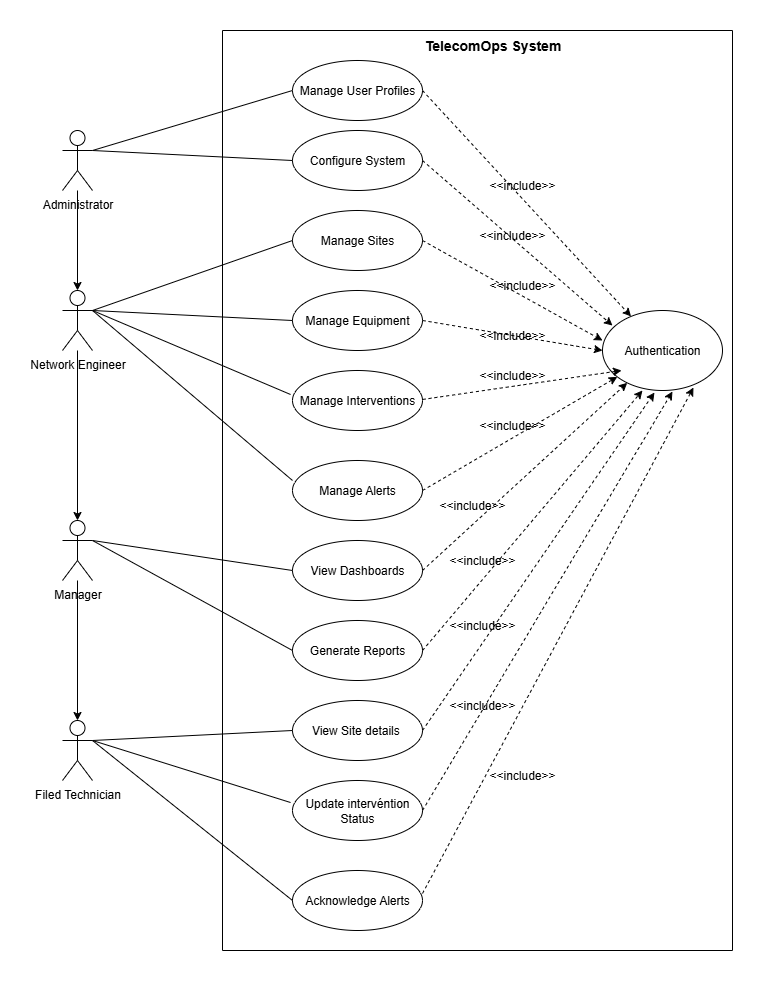
\includegraphics[width=0.95\linewidth]{img/chap_02/TelecomOps_UseCase_Diagram.png}
    \caption{TelecomOps Global Use Case Diagram}
    \label{fig:use_case_global}
\end{figure}

The global use case diagram illustrates comprehensive interaction patterns between stakeholder types and system functionalities, providing visual representation of system scope and user accessibility patterns. The diagram employs role inheritance demonstrating permission escalation: Field Technicians possess base operational capabilities including viewing assigned interventions, updating statuses, and reporting breakdowns. Managers inherit all technician capabilities while adding supervisory functions including viewing statistics, creating sites, scheduling interventions, and analyzing performance. Network Engineers inherit manager capabilities while adding technical functions including root cause analysis, equipment specification management, and detailed technical planning. Administrators inherit all engineer capabilities while adding exclusive system management functions including user management, system configuration, and data deletion.

This hierarchical structure reflects operational reality where higher roles need all capabilities of lower roles to effectively supervise and support their teams. The comprehensive coverage demonstrates system addresses all stakeholder needs identified in Section 2.2 through specific capabilities.

Detailed use case specifications for each functional module are presented in corresponding sprint implementation chapters (Chapters 3 through 7) where they are examined in context of specific development iterations with comprehensive scenario analysis, sequence diagrams, and validation procedures. This organization prevents redundancy while ensuring use cases receive appropriate technical depth when implementation details are available.

\section{System Architecture}

The TelecomOps system architecture implements modern, scalable design addressing complex requirements of telecommunications infrastructure management while ensuring security, performance, and maintainability.

\subsection{Architectural Overview}

The system follows layered architecture pattern organized into three distinct tiers providing clear separation of concerns and enabling independent scaling of components.

\begin{figure}[H]
    \centering
    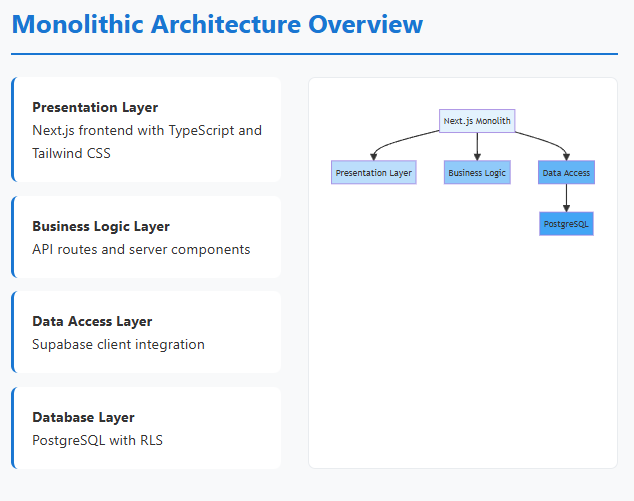
\includegraphics[width=0.7\linewidth]{img/chap_02/architecture_overview.png}
    \caption{TelecomOps System Architecture Overview}
    \label{fig:architecture_overview}
\end{figure}

The system architecture overview diagram illustrates the layered approach: the presentation layer handles user interface and interactions providing responsive user experience across devices; the application layer manages business logic and backend services coordinating data access and enforcing business rules; and the data layer provides persistent storage and data management ensuring data integrity and consistency.

This separation ensures modularity where each layer can evolve independently, maintainability through clear component boundaries, and scalability through independent tier scaling based on specific load patterns. The architecture emphasizes loose coupling between layers enabling independent evolution and testing, clear interfaces between components facilitating future enhancement, and security through defense-in-depth with protection at multiple levels.

\subsubsection{Presentation Layer}

The presentation layer implements responsive, progressive web application using modern frontend technologies delivering exceptional user experience across all devices and screen sizes.

\textbf{Technology Stack:} Next.js 14 (React framework with server-side rendering and automatic code splitting), TypeScript (type-safe development with compile-time checking), Tailwind CSS (utility-first styling with minimal production bundle), and Shadcn/UI (accessible component library with WCAG compliance).

\textbf{Key Capabilities:} Responsive design supporting desktop, tablet, and mobile devices; Progressive Web App features including offline capabilities; server-side rendering for improved performance; real-time data updates through WebSocket connections; and optimized asset delivery via CDN distribution.

\subsubsection{Application Layer}

The application layer provides comprehensive backend services through Supabase Backend-as-a-Service platform offering authentication, data management, and real-time capabilities.

\textbf{Core Services:} Authentication Service (JWT tokens with role-based access control), Database API (auto-generated RESTful endpoints from PostgreSQL schema), Real-time Engine (WebSocket subscriptions for live updates), Storage Service (file management for documentation and media), and Edge Functions (serverless computing for custom logic).

\subsubsection{Data Layer}

The data layer implements robust PostgreSQL database with advanced security and performance features optimized for telecommunications operations.

\textbf{Database Features:} Row Level Security (fine-grained access control at database level), JSONB Support (flexible storage for complex specifications), Full-text Search (advanced search across multiple data types), Automated Backups (point-in-time recovery capabilities), and Connection Pooling (optimized resource utilization for high concurrency).

\subsection{Global Class diagram}

The database schema implements normalized relational design optimized for telecommunications operations while maintaining flexibility for future enhancements.

\begin{figure}[H]
    \centering
    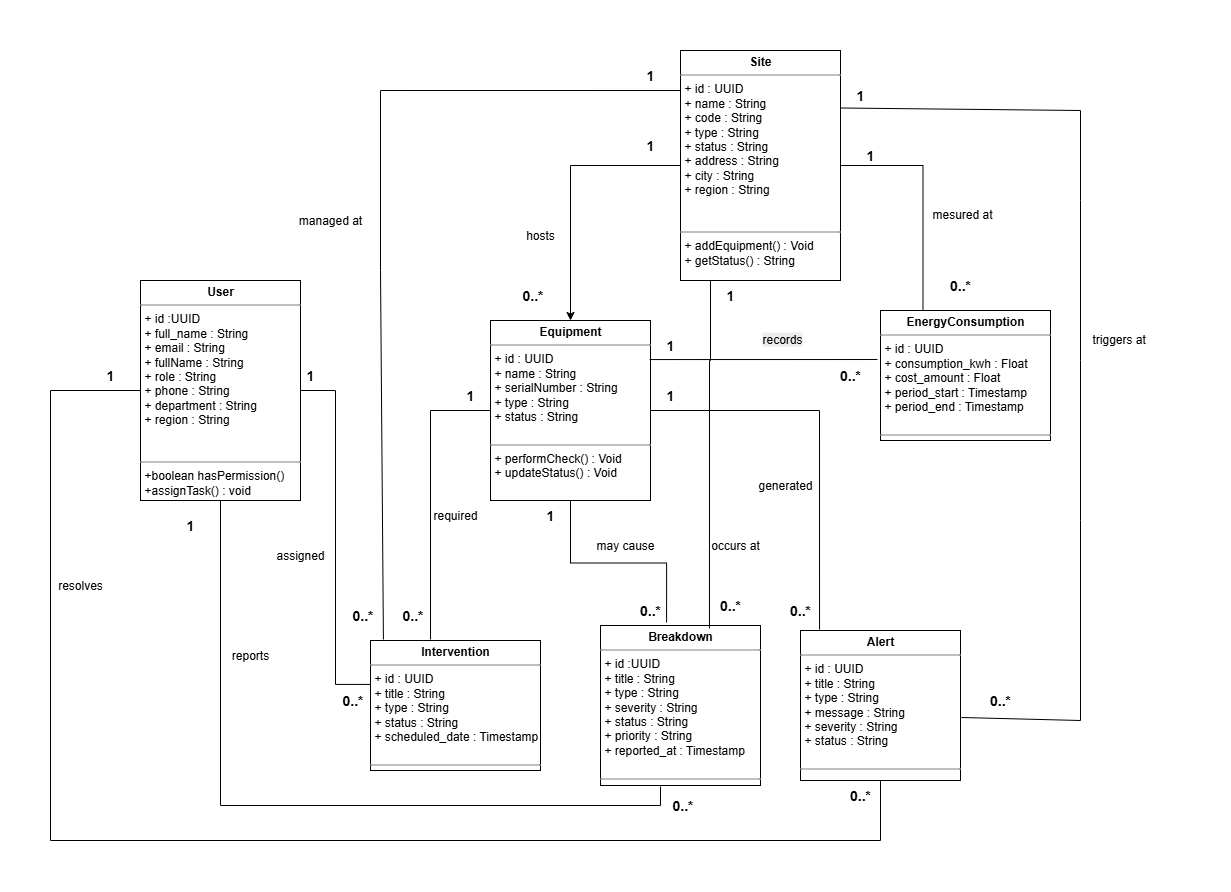
\includegraphics[width=1\linewidth]{img/chap_02/database_er_diagram.png}
    \caption{Global Class Diagram}
    \label{fig:database_er_diagram}
\end{figure}

The entity-relationship diagram illustrates core database entities and relationships forming cohesive data model supporting all system operations. The schema design reflects clear entity boundaries with single responsibility, explicit foreign key relationships ensuring referential integrity, appropriate constraints enforcing data validity, and flexible JSONB storage for semi-structured data.

\subsubsection{Core Entities}

\textbf{Profiles:} User information linked to Supabase authentication with role assignment (admin, engineer, technician, manager), region for geographical access control, and timestamps for audit trails.

\textbf{Sites:} Telecommunications locations with unique site codes, geographical coordinates stored as JSONB, network technologies (2G/3G/4G/5G) as array, operational status with workflow states, and maintenance schedule timestamps.

\textbf{Equipment:} Network hardware inventory with unique serial numbers, equipment type classification, brand and model information, technical specifications in JSONB format, installation and warranty dates, and operational status with change tracking.

\textbf{Interventions:} Maintenance activities with site and optional equipment associations, assigned technician reference, intervention type and priority classification, scheduled and completed timestamps, and technician notes documenting work performed.

\textbf{Breakdowns:} Fault reports with severity classification (minor, major, critical), impact assessment including affected users, downtime tracking with automatic duration calculation, status workflow management, and resolution documentation.

\textbf{Alerts:} System notifications with severity levels (info, warning, critical), alert type classification, site and equipment associations, status workflow (active, acknowledged, resolved), and user tracking for creation, acknowledgment, and resolution.

\textbf{Energy Consumption:} Power usage records with kWh measurements, automated cost calculations based on configurable rates, period definitions (daily, weekly, monthly), threshold validation for anomaly detection, and site/equipment associations for granular analysis.

\subsection{Security Architecture}

Security implementation follows defense-in-depth principles with multiple protection layers ensuring data confidentiality, integrity, and availability.

\begin{figure}[H]
    \centering
    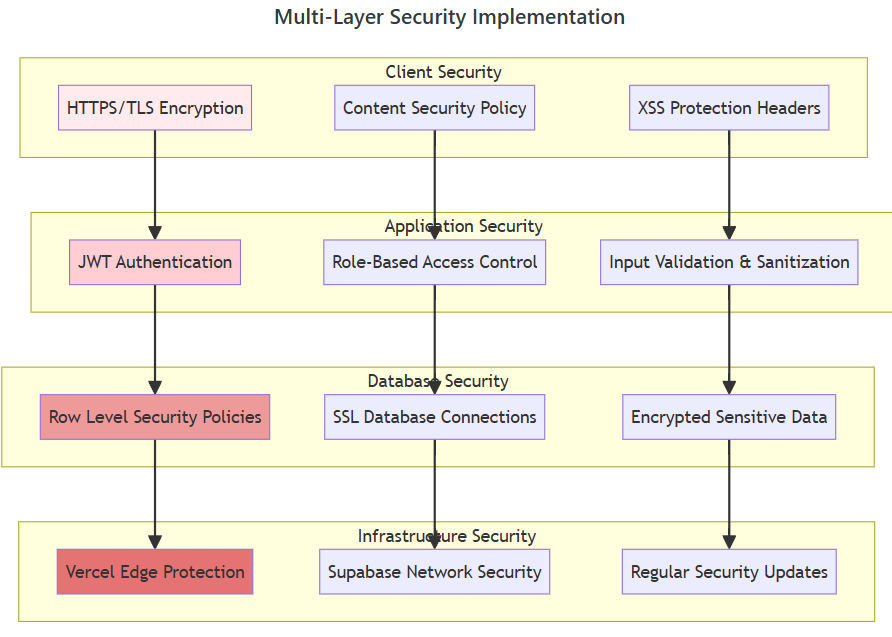
\includegraphics[width=1\linewidth]{img/chap_02/security_architecture.png}
    \caption{Multi-Layer Security Architecture}
    \label{fig:security_architecture}
\end{figure}

The security architecture implements four distinct layers each addressing specific threat vectors and providing independent protection:

\textbf{Transport Security:} TLS 1.3 encryption for all communication, HSTS headers forcing HTTPS, Content Security Policy preventing XSS attacks, and secure cookie flags (Secure, HttpOnly, SameSite).

\textbf{Application Security:} JWT-based authentication with configurable expiration, role-based access control with granular permissions, API rate limiting preventing abuse, comprehensive input validation using Zod schemas, and CSRF protection on state-changing operations.

\textbf{Database Security:} Row Level Security policies enforcing role-based data access, encryption at rest using AES-256, connection encryption via SSL/TLS, comprehensive audit logging tracking all modifications, and prepared statements preventing SQL injection.

\textbf{Infrastructure Security:} Web Application Firewall protecting against common attacks, DDoS mitigation through cloud protection, network isolation with controlled access, automated security monitoring detecting unusual patterns, and regular security updates through managed services.

\section{Technology Stack Justification}

Technology selection prioritizes reliability, scalability, security, and development efficiency while ensuring alignment with modern practices and telecommunications requirements.

\subsection{Frontend Technologies}

\textbf{Next.js 14:} React framework providing server-side rendering, automatic code splitting, and production optimizations. Selected for performance through SSR and code splitting, development experience with hot reloading and comprehensive tooling, and production readiness with automatic optimizations.

\textbf{TypeScript:} Type-safe JavaScript superset ensuring code reliability through compile-time error detection. Chosen for self-documenting code reducing onboarding time, superior IDE support with autocompletion and refactoring, and improved maintainability through type-safe refactoring.

\textbf{Tailwind CSS:} Utility-first CSS framework enabling rapid interface development with consistent design tokens. Selected for exceptional development speed through utility composition, guaranteed design consistency via predefined scales, and minimal production bundles through automatic purging.

\textbf{Shadcn/UI:} Accessible component library built on Radix UI primitives maintaining WCAG standards. Chosen for accessibility compliance meeting NFR-006, customizable components matching telecommunications requirements, and seamless Tailwind CSS integration.

\textbf{React Query:} Data fetching library with intelligent caching and automatic refetching. Selected for declarative data fetching patterns, built-in loading and error states, optimistic updates improving perceived performance, and powerful cache management reducing network requests.

\textbf{Zustand:} Lightweight state management with minimal boilerplate. Chosen for straightforward API with minimal configuration, excellent TypeScript support with full type inference, and minimal bundle size impact addressing performance requirements.

\subsection{Backend Technologies}

\textbf{Supabase:} Open-source Backend-as-a-Service built on PostgreSQL. Selected for PostgreSQL foundation ensuring ACID compliance, built-in Row Level Security enabling fine-grained access control, real-time capabilities via WebSocket, managed infrastructure reducing operational overhead, and open-source architecture preventing vendor lock-in.

\textbf{PostgreSQL:} Enterprise-grade relational database with proven reliability. Chosen for ACID compliance ensuring data consistency in mission-critical operations, JSONB support providing flexible semi-structured storage, full-text search enabling advanced queries, mature query optimizer supporting high-performance operations, and rich extension ecosystem for specialized requirements.

\textbf{PostgREST:} Automatic REST API generator from PostgreSQL schema. Selected for instant API generation reducing backend development time, automatic endpoint creation based on schema, and security through database-level access control policies.

\subsection{Development and Deployment Tools}

\textbf{Git and GitHub:} Version control system and repository hosting. Essential for team coordination, maintaining complete project history, automated CI/CD triggers, code review workflows, and integrated issue tracking.

\textbf{Docker:} Containerization platform ensuring environment consistency. Utilized for development environment standardization, reproducible builds through versioned images, and deployment flexibility for infrastructure requirements.

\textbf{Node.js:} JavaScript runtime for server-side execution. Selected for consistent environment across development and production, comprehensive npm package ecosystem, and optimized performance for I/O-intensive operations.

\textbf{Jenkins:} Automation server for CI/CD pipelines. Chosen for extensive plugin ecosystem supporting Docker and Git workflows, pipeline-as-code enabling version control, and distributed builds supporting parallel execution.

\textbf{Kubernetes:} Container orchestration platform for deployment management. Selected for automated deployment and scaling, service discovery and load balancing, self-healing capabilities with automatic restart, and declarative configuration enabling infrastructure as code.

\subsection{Additional Libraries}

\textbf{Recharts:} React charting library for data visualization. Selected for composable architecture matching React patterns, responsive design adapting to screen sizes, and extensive customization for telecommunications-specific visualizations.

\textbf{jsPDF:} Client-side PDF generation library. Chosen for browser-based generation reducing server load, comprehensive formatting capabilities, and UTF-8 support for multilingual content.

\textbf{Lucide React:} Icon library with consistent design. Selected for extensive icon collection, tree-shakeable architecture minimizing bundle size, and TypeScript support with full definitions.

\textbf{Date-fns:} Date manipulation library. Chosen for modular architecture allowing selective imports, immutable approach preventing side effects, and extensive locale support for internationalization.

\textbf{Zod:} TypeScript-first schema validation. Selected for TypeScript-first design with automatic type inference, comprehensive validation rules, clear error messages, and runtime type safety.

\section{Deployment Architecture}

The deployment architecture implements automated DevOps pipeline leveraging containerization and orchestration technologies ensuring reliable, scalable production deployments.

\begin{figure}[H]
    \centering
    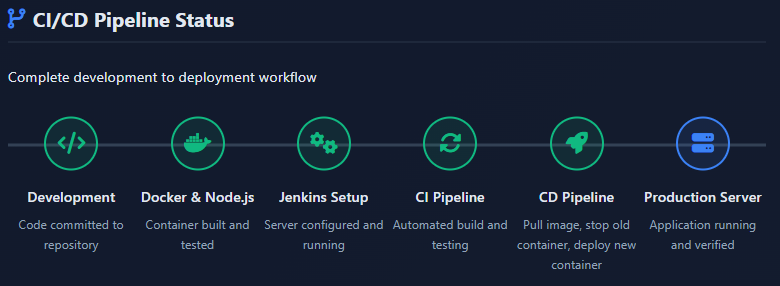
\includegraphics[width=0.9\linewidth]{img/chap_02/deployment_architecture.png}
    \caption{Global Deployment Architecture}
    \label{fig:deployment_architecture}
\end{figure}

The deployment architecture diagram illustrates the complete infrastructure topology from development environment through continuous integration and deployment to production Kubernetes cluster. The architecture demonstrates the flow from code commit triggering automated build processes, through containerization and testing, to orchestrated deployment across distributed infrastructure.

\subsection{Development Environment Configuration}

\textbf{VM Creation (Ubuntu):} Virtual machine provisioned with Ubuntu Server 22.04 LTS providing isolated development and build environment. The VM configuration includes adequate resources (4 CPU cores, 8GB RAM, 100GB storage) supporting Docker containerization and Jenkins execution, network configuration enabling external access to Jenkins web interface, and security hardening following Ubuntu server best practices.

\textbf{Docker Installation:} Container runtime installed using official Docker repository ensuring latest stable version. Docker provides application containerization enabling consistent environments across development, testing, and production stages, isolated execution preventing dependency conflicts, and efficient resource utilization through shared kernel architecture.

\textbf{Node.js Installation:} Node.js runtime (version 18 LTS) installed via NodeSource repository enabling JavaScript execution for Next.js application. Node.js provides consistent JavaScript runtime environment, npm package manager for dependency management, and optimized V8 engine for application performance.

\subsection{Containerization Strategy}

\textbf{Dockerfile Creation:} Multi-stage Dockerfile created defining application containerization process. The Dockerfile implements build stage installing dependencies and compiling Next.js application, production stage with minimal runtime dependencies reducing image size, and optimized layer caching accelerating subsequent builds through intelligent layer reuse.

\textbf{Docker Image Testing:} Comprehensive testing validates containerized application before deployment. Testing includes container build verification ensuring successful compilation, runtime testing confirming application starts and responds correctly, and resource utilization monitoring ensuring efficient memory and CPU usage within container constraints.

\subsection{CI/CD Infrastructure}

\textbf{Jenkins in Docker:} Jenkins automation server deployed as Docker container ensuring reproducible Jenkins environment and simplified management. Container deployment provides persistent Jenkins configuration through volume mounting, isolated execution preventing conflicts with host system, and straightforward version upgrades through container image updates.

\textbf{Jenkins Server Configuration:} Initial Jenkins setup includes plugin installation (Docker, Git, Pipeline, Credentials), user account creation with appropriate permissions for pipeline management, and credentials configuration securely storing Docker Hub authentication tokens and deployment keys.

\subsection{Continuous Integration Pipeline}

\textbf{CI Pipeline Implementation:} Automated pipeline triggered on Git commits performs comprehensive build and test operations. The pipeline stages include source code checkout from GitHub repository, dependency installation using npm with caching for efficiency, TypeScript compilation verifying type safety, ESLint validation ensuring code quality standards, unit test execution confirming component functionality, Docker image build creating production-ready container, and image push to Docker Hub registry with semantic versioning tags.

\subsection{Continuous Deployment Pipeline}

\textbf{CD Pipeline Implementation:} Automated deployment pipeline triggered on successful CI completion deploys application to target environments. The pipeline stages include Docker image pull from registry retrieving latest validated build, environment-specific configuration injection providing appropriate credentials and settings, container deployment to Kubernetes cluster using kubectl commands, health check validation confirming successful deployment, and automated rollback on failure ensuring service continuity.

\subsection{Container Orchestration}

\textbf{Kubernetes Configuration:} Container orchestration platform manages application deployment across distributed infrastructure. Kubernetes provides deployment manifests defining desired application state with replica count and resource limits, service definitions exposing application through load balancer, ingress configuration routing external traffic to appropriate services, persistent volume claims ensuring data persistence across pod restarts, and horizontal pod autoscaling automatically adjusting replica count based on CPU/memory utilization.

\subsection{Monitoring and Operations}

\textbf{Application Monitoring:} Comprehensive monitoring tracks application health and performance. Monitoring includes container health checks ensuring pods respond to liveness and readiness probes, resource utilization tracking CPU and memory consumption, application logs aggregated centrally for troubleshooting, and performance metrics collecting response times and error rates.

\textbf{Infrastructure Monitoring:} Kubernetes cluster monitoring ensures infrastructure health. Infrastructure monitoring tracks node resource availability, pod scheduling and status, network connectivity and traffic patterns, and storage utilization and performance.

This deployment architecture, detailed comprehensively in Sprint 6 (Chapter 8), provides production-ready infrastructure supporting TelecomOps operational requirements while enabling automated, reliable deployments through proven DevOps practices.

\section*{Conclusion}

This chapter established comprehensive planning and architectural foundation for TelecomOps project. Through stakeholder analysis, we identified four distinct user roles with specific operational requirements driving system design decisions. The enhanced Manager role with site creation and status management capabilities reflects operational reality of deployment approval and operational decision-making.

Requirements specification defined 9 functional requirements covering authentication, site management, equipment inventory, interventions, breakdowns, alerts, energy monitoring, and reporting, along with 6 non-functional requirements ensuring performance, scalability, security, reliability, and usability. The product backlog with 22 granular user stories provides clear development roadmap enabling focused development and incremental delivery.

The six-sprint Scrum approach ensures iterative value delivery building systematically from authentication and site management through equipment inventory, operational processes, monitoring capabilities, analytics, and production deployment. Each sprint has clear objectives and measurable success criteria enabling objective completion assessment.

The system architecture implementing layered approach with Next.js frontend, Supabase backend, and PostgreSQL database provides modern, scalable foundation. The comprehensive security architecture with four protection layers ensures data confidentiality and integrity through defense-in-depth principles. Technology selection throughout prioritizes proven solutions balancing development efficiency with operational reliability.

The deployment architecture leveraging Docker containerization, Jenkins automation, and Kubernetes orchestration provides automated DevOps pipeline ensuring reliable, scalable production deployments. This infrastructure, detailed in Sprint 6, demonstrates enterprise-ready deployment practices appropriate for mission-critical telecommunications operations.

This foundation provides clear requirements, sprint organization, architectural design, and technology justification positioning the project for systematic implementation addressing Tunisie Telecom's operational needs. Following chapters detail sprint-by-sprint implementation demonstrating how planning translates into operational telecommunications management solution, with each sprint chapter presenting detailed use case specifications, sequence diagrams, implementation screenshots, technical challenges and solutions, and comprehensive testing validation.